\documentclass[final,a4j,12pt]{jreport}
\newfont {\boldmathl}{cmmib10 scaled\magstep1}
\newcommand{\bm}[1]{\mbox{\boldmathl #1}}
\newcommand{\lw}[1]{\smash{\lower2.0ex\hbox{#1}}}

\usepackage{multicol}
\usepackage{amsmath,amssymb}
\usepackage{here}
\usepackage{bm}

\usepackage[dvipdfmx]{graphicx}
\usepackage{textcomp}
\usepackage{plext}
\usepackage{enumerate}
\usepackage{epsfig}
\usepackage{comment}
\usepackage{longtable}
\usepackage{./stylefile/cite}
\usepackage{./stylefile/jverb}
\usepackage{./stylefile/here}
\usepackage{./stylefile/bpaper}
\usepackage{./stylefile/epsbox}
\usepackage{./stylefile/fancyheadings}
\usepackage{./stylefile/slashbox}
\usepackage{./stylefile/subfigure}
\bibliographystyle{./stylefile/jecon}

\def\frac#1#2{\genfrac{}{}{}{}{\;#1\;}{\;#2\;}}
\def\dfrac#1#2{\genfrac{}{}{}{0}{\;#1\;}{\;#2\;}}
\def\tfrac#1#2{\genfrac{}{}{}{1}{\;#1\;}{\;#2\;}}
\def\sfrac#1#2{\genfrac{}{}{}{2}{\;#1\;}{\;#2\;}}
\def\ssfrac#1#2{\genfrac{}{}{}{3}{\;#1\;}{\;#2\;}}

\usepackage{tabularx}
\newcolumntype{Y}{>{\centering\arraybackslash}X}
\newcolumntype{Z}{>{\raggedleft\arraybackslash}X}

\usepackage{url}
\renewcommand{\url}{\begingroup \def\UrlLeft{}\def\UrlRight{}\urlstyle{rm}\Url}

\def\so{.\raisebox{1ex}{.}.\quad}
\def\because{\raisebox{1ex}{.}.\raisebox{1ex}{.}\quad}
\def\Omicron{O}
\def\omicron{o}

\newcommand{\pdif}[2]{\frac{\partial #1}{\partial #2}}

\setcounter{secnumdepth}{6}
\makeatletter
\newcommand{\subsubsubsection}{\@startsection{paragraph}{4}{\z@}
  {1.5\Cvs \@plus.5\Cdp \@minus.2\Cdp}
  {.5\Cvs \@plus.3\Cdp}
  {\reset@font\normalsize\sffamily}
}

\def\bs#1{\boldsymbol{#1}}
\def\quot#1{``#1''}
\def\ggn{Google {\it N}-gram}


\addtolength{\topmargin}{-15mm}
\addtolength{\oddsidemargin}{-15mm}


\begin{document}
\begin{titlepage}
\thesis
{時間軸セグメントを導入した \\ 階層的時間記憶モデル}
{Hierarchical Temporal Memory with \\ time axis segment introduced}
{萩原 将文 教授}
{西 宏章 教授}
{29}
{学籍番号 61412912}
{内藤 慎一郎}
\end{titlepage}
\pagenumbering{roman}

\contents

\pagenumbering{arabic}


% \abstract
本論文では大脳皮質の構造と学習アルゴリズムを模した時系列予測モデルであるHierarchical Temporal Memory(HTM)に長期依存考慮に関する改良を加えることを提案する。
HTMは脳の神経細胞を表すセルを2次元マップ上に配置し、各セル間を繋げるシナプス接続をヘブ則に基づいて更新することで時系列データを学習する。
従来のモデルでは時系列データ中の各データに対して一時刻前のデータとの接続のみを学習していたが、本研究では複数時刻前のデータとの接続を学習させることを目的とした。
そのためにシナプスの集まりであるセグメントに対して時間軸を導入したモデルを提案した。
これによって様々な時系列データの予測タスクにおいて従来モデルよりも高い精度を記録することを確認した。

% \chapter{はじめに}
近年、深層学習という多層に重ねたニューラルネットワークにおいて目的関数の誤差を減少させる
ことで最適化を行うモデルが様々なタスクで成果をあげている。
その中でもRNN, LSTMといった時系列データを扱うモデルが自然言語処理や音声認識といった幅広い分野に用いられている。

しかし人間の脳における大脳皮質の学習は目的関数に対して最適化するという学習をおこなっているのではないとされている。\cite{neurons}
人間の脳における学習はニューロンが発火していくことによるニューロン間をつなぐシナプスの発生によって行われる。
この学習を模したニューラルネットワークモデルとしてHierarchical Temporal Memory(HTM)が提案された。\cite{htm}

HTMの構造や学習アルゴリズムは人間の脳の大脳皮質を模したものとなっている。
HTMの構造は神経細胞を模したセルと名付けなれたノードを2次元マップ状に配置したものとなっている。
またそのセルはそれぞれ非活性化状態、予測状態、活性化状態と遷移するようになっている。
学習アルゴリズムはそのセル間の繋がりであるシナプス接続の可否を変化させるというものである。
シナプス接続の可否は各シナプスの接続値を増減させることで変化させるが、それはヘブ則によって行われる。これはあるセルの発火の後に他のセルが発火した時にその2つのセル間のシナプス接続が強化させるというものである。

HTMはシナプス接続を元にして活性化状態のセルと繋がっているセルが予測状態に遷移し、次の時刻に置いて予測状態のセルが活性化状態に遷移することで時系列データを再現しようとする。
HTMはこのシナプス接続を束ねたものとしてセグメントという機構があるが、これは神経細胞の樹状突起を模したものである。またこのセグメントは1つのセルに対して複数あるためセグメント集合となる。

またHTMの学習は深層学習でよく用いられるミニバッチ学習とは異なり、1つ1つのデータの入力に対して学習を更新するオンライン学習となっている。
また目的関数に対して最適化を行うのではないため教師なし学習に分類される。

他のHTMの特徴として疎な分散表現が挙げられる。マップ状になったセルの内わずかなセルのみが発火してデータを表現するため少ない計算量と幅広い表現力を持っている。

HTMは深層学習におけるニューラルネットワークに対してわずかなタスクにおいては優位性があるが、ほとんどのタスクにおいて低い精度となっている。
また自然言語処理などの複雑なタスクには用いられていない。
特にRNNに長期依存考慮のためのゲート機構を導入したLSTMのような高度な時系列予測が行えていない。

この原因としてHTMには長期依存考慮のための機構が加えられていないことが考えられる。
特に疎な分散表現による学習が続けられていくによって発火するセルが減少する。
これによって予測情報が維持できなくなり、長期依存関係が消失する。

そのため本研究ではHTMのセグメント集合に対して時間軸を導入し、複数前の時刻におけるデータを表現しているセルとの繋がりも学習可能なモデルを構築した。
これによって疎な分散表現を維持しつつも長期依存関係の学習を目指す。
またHTMの学習アルゴリズムを改良した研究というものは現在挙げられていない。

本研究の評価として様々な時系列データの予測タスクにおいて従来のHTMとの比較を行った。

以下、第2章でHTMの構造と学習アルゴリズムについて詳しく述べ、第3章で改良したHTMについて、第4章で評価実験、第5章で結論を述べる。

% \chapter{�w�K�E�e�X�g�f�[�^�̍쐬}

\section{�g�p�f�[�^�Z�b�g}

��ăV�X�e���ɂ����Ċw�K��e�X�g�ɗp����摜�ɂ́CCelebA�f�[�^�Z�b�g\cite{liu2015faceattributes}���g�p�����D���̃f�[�^�Z�b�g�́C�����l�̊�摜20��2599�����琬��f�[�^�Z�b�g�ŁC40��ނ̑������x�����e�摜�ɕt������Ă���D�摜�����ɂ͑�ʂ̉摜���K�v�ł���C�܂��C������񂪕t�^����Ă���f�[�^�Z�b�g���K�v�ł��邽��CelebA�f�[�^�Z�b�g���g�p�����D
%http://mmlab.ie.cuhk.edu.hk/projects/CelebA.html

\section{�摜�̃��T�C�Y}
�g�p����CelebA�f�[�^�Z�b�g�̉摜�T�C�Y��178$\times$218pixels�ł���D�摜�̓����ʂ𒊏o����VGG-19�l�b�g���[�N�͓��͂Ƃ���摜�̃T�C�Y��224$\times$224pixels�Ɍ��肳��Ă��邽�߁CCelebA�f�[�^�Z�b�g�̉摜�����T�C�Y����K�v������D�s���������̗����}\ref{fig:resize}�Ɏ����D

\begin{figure}[H]
 \begin{center}
  \includegraphics[scale=0.5]{./fig/resize.eps}
  \caption{�摜�T�C�Y�����̗���}
  \label{fig:resize}
 \end{center}
\end{figure}


\begin{description}
\item[1�D�����`�ɐ؂���.]\mbox{}\\ 
���s���ʂ̗��}\ref{fig:crop}�Ɏ����DCelebA�f�[�^�Z�b�g���̉摜�͊炪�摜�̒��S�ɂ�����̂��������߁C�㉺20pixel��؂���C178$\times$178pixels�̉摜���쐬�����D��̗̈�𐳊m�ɐ؂�����@�Ƃ��āC�猟�o���s���C���̗̈��؂��鎖���l���������C�猟�o�𐳂����s���Ȃ������ꍇ�̑Ώ��ɂ������Ԃ�C�����؂����Ă��܂����ő�����񂪎����Ă��܂��”\�����l���C�P���ɏ㉺20pixel��؂�����@��I�������D

\begin{figure}[H]
 \begin{center}
  \includegraphics[scale=0.7]{./fig/crop.eps}
  \caption{�؂�����@�̈Ⴂ}
  \label{fig:crop}
 \end{center}
\end{figure}

\item[2�DCl-waifu2x�𗘗p���ĉ𑜓x�����킸�Ɋg�傷��.]\mbox{}\\ 
���s���ʂ̗��}\ref{fig:waifu2x}�Ɏ����D178$\times$178pixels�̉摜�����̂܂�224$\times$224pixels�Ƀ��T�C�Y���Ă��܂��ƁC�𑜓x�������Ă��܂����߁C�𑜓x��ۂ����܂܉摜���g�傷�鎖���o����Cl-waifu2x\cite{waifu2x}�Ƃ����V�X�e���𗘗p�����DCl-waifu2x�Ƃ́COpenCL��p���Ď������ꂽ�C�𑜓x��ۂ����܂�2�{�̑傫���ɉ摜���g�傷�鎖���o����V�X�e���ł���D����ɂ��C�摜�T�C�Y��356$\times$356pixels�ƂȂ�D
%https://github.com/marcan/cl-waifu2x
\begin{figure}[H]
 \begin{center}
  \includegraphics[scale=0.5]{./fig/waifu2x.eps}
  \caption{waifu2x�ɂ��g��}
  \label{fig:waifu2x}
 \end{center}
\end{figure}


\item[3�D224$\times$224pixels�ɏk������D]\mbox{}\\  
���s���ʂ̗��}\ref{fig:small}�Ɏ����D�쐬����356$\times$356pixels�̉摜���CVGG-19�l�b�g���[�N�ɓ��͂ł���悤��224$\times$224pixels�ɏk�������D
\begin{figure}[H]
 \begin{center}
  \includegraphics[scale=0.2]{./fig/small.eps}
  \caption{�k��}
  \label{fig:small}
 \end{center}
\end{figure}
\end{description}

\section{���������E�����Ȃ��摜�g�̒��o}
����͕t�^���鑮���Ƃ��āA�Ί�̗�œ��o�̓f�[�^�̒��o���@�ɂ‚��ďq�ׂ�D��ă��f�����w�K�E�e�X�g���邽�߂ɂ́C�Ί�E�Ί�ł͂Ȃ��摜�̑g����萔�K�v�ƂȂ�C���̉摜�g��p���ĕt�^���鑮�������ʂ𐶐�����D���̏Ί�E�Ί�ł͂Ȃ��摜�̑g�𒊏o������@�Ƃ��Ď���5�p�^�[�����l�����D

\begin{description}
\item[1�DCelebA�f�[�^�Z�b�g�ɕt�����Ă��郉�x������p������@]\mbox{}\\ 
�}\ref{fig:listattr}�ɁCCelebA�f�[�^�Z�b�g�ɕt�����Ă���hlist\_attr\_celeba.txt�h�Ƃ����e�L�X�g�t�@�C���̈ꕔ������.�e�L�X�g�t�@�C���Ƀ��x����񂪋L������Ă���C�e�����ɂ��Ă͂܂�ꍇ�Ɂh1�h�C���Ă͂܂�Ȃ��ꍇ�Ɂh-1�h���L�����Ă���D �������C�}\ref{fig:listattr}�̏�i�̐����͑����ԍ��������D�{���̃e�L�X�g�t�@�C���ɂ͑��������L�q����Ă��邪�C�ȗ��̂��ߔԍ��ŕ\�����D���̃e�L�X�g�t�@�C����p���āC�Ί瑮�����قȂ�C��39�����������摜�̑g�𒊏o����D���o�A���S���Y����}\ref{fig:overlap}�Ɏ����D

\begin{figure}[H]
 	\begin{center}
 		\includegraphics[scale=0.4]{./fig/listattr.eps}
 		\caption{�hlist\_attr\_celeba.txt�h�̈ꕔ}
 		\label{fig:listattr}
 	\end{center}
 \end{figure}
 \begin{figure}[H]
 	\begin{center}
 		\includegraphics[scale=0.6]{./fig/overlap.eps}
 		\caption{���x������p�������o���@}
 		\label{fig:overlap}
 	\end{center}
 \end{figure}
 
���̒��o���@�ɂ�蒊�o���ꂽ�摜�g�̗��}\ref{fig:imageoverlap}�Ɏ����D
\begin{figure}[H]
 	\begin{center}
 		\includegraphics[scale=0.25]{./fig/imageoverlap.eps}
 		\caption{���o�����摜��}
 		\label{fig:imageoverlap}
 	\end{center}
 \end{figure}

���̒��o���@�ł́C���x�����ގ����Ă���摜���I���ł������ŁC�}\ref{fig:imageoverlap}��2�C3�̗���݂�ƕ�����悤�ɁC1���̉摜�ɑ΂��ĕ����̉摜���Ή����Ă��܂��ꍇ������D

\item[2�D1.�Œ��o�����摜�y�A����d�����폜������@]\mbox{}\\ 
��ŏq�ׂ��悤�ɁC1.�̒��o���@�ł́C1���̉摜�ɑ΂��ĕ����̉摜���Ή����Ă��܂��ꍇ������D���̂悤�ȏꍇ�C��������摜������̉摜�ɗގ����Ă��܂��Ȃǂ̖��_����������D���̂��߁C1.�Œ��o�����摜�g�̒����烉���_���ɏd������摜�g���폜�����D���o�A���S���Y����}\ref{fig:removeoverlap}�Ɏ����D
\begin{figure}[H]
 	\begin{center}
 		\includegraphics[scale=0.6]{./fig/removeoverlap.eps}
 		\caption{�d������摜�g�̍폜���@}
 		\label{fig:removeoverlap}
 	\end{center}
 \end{figure}

\item[3�D�摜�̗ގ��x��p������@]\mbox{}\\ 
1.�̕��@�Œ��o�����摜�g�́C���x�����ގ����Ă���摜���I���”\�ł��邪�C��̌�����w�i�F�Ȃǂ̃��x�����ȊO�̗v�f���傫���قȂ�摜���I������Ă��܂��Ƃ������_������D�����ŁC�摜�̗ގ��x���l�������Ί�E�Ί�ł͂Ȃ��摜�g�̒��o���@���l�����D���o�A���S���Y����}\ref{fig:cossim}�Ɏ����D �܂�CelebA�f�[�^�Z�b�g�̑S�Ẳ摜���Ί�̉摜�Q�C�Ί�ł͂Ȃ��摜�Q�ɕ�������D���������Ί�̉摜�Q1���ɑ΂��C�Ί�ł͂Ȃ��摜�Q�̑S�Ẳ摜�Ƃ̗ގ��x���v�Z���C�ގ��x��1�ԍ����摜��I������D�摜�̗ގ��x�v�Z�ɂ̓R�T�C���ގ��x���g�p�����D�����������摜(�Ί�摜)��$\bm{x}^t$�C���͉摜(�Ί�ł͂Ȃ��摜)��$\bm{x}^s$�Ƃ���D�R�T�C���ގ��x�ɂ��摜�̗ގ��x��
\begin{equation}
  cos(\bm{x}^t, \bm{x}^s) = \frac{\bm{x}^t \cdot \bm{x}^s}{|\bm{x}^t||\bm{x}^s|}
\end{equation}
�ƌv�Z�ł���.
�摜��ǂݍ���RGB�l�̍s���1�����̃x�N�g���ɕϊ����C�R�T�C���ގ��x�̌v�Z���s�����D
\begin{figure}[H]
 	\begin{center}
 		\includegraphics[scale=0.6]{./fig/cossim.eps}
 		\caption{�摜�̗ގ��x�ɂ�钊�o���@}
 		\label{fig:cossim}
 	\end{center}
 \end{figure}

���̒��o���@�ɂ�蒊�o���ꂽ�摜�g�̗��}\ref{fig:imagecossim}�Ɏ����D
\begin{figure}[H]
 	\begin{center}
 		\includegraphics[scale=0.25]{./fig/imagecossim.eps}
 		\caption{���o�����摜��}
 		\label{fig:imagecossim}
 	\end{center}
 \end{figure}

�������C���̒��o���@�ł͏d������摜�����݂���”\��������Ƃ������_������D�܂��C�w�i���̌����Ȃǂ��l�������摜�y�A�𒊏o�ł������ŁC�}\ref{fig:imagecossim}��3�̂悤�ɁC�Ί�ȊO�̑����̈قȂ�摜�y�A��I�����Ă��܂��Ƃ������_�����݂���D�������C�Ί瑮���Ɋ܂܂��摜�̐������摜�g�𒊏o�ł��邽�߁C���̒��o���@�ɔ�ׂđ�K�͂ȉ摜�g���쐬�ł���D

\item[4�D1.�Œ��o�����摜�y�A����摜�̗ގ��x�𗘗p���ďd�����폜������@]\mbox{}\\ 
�ȏ�̃p�^�[�����l�����C1.�Œ��o�����摜�y�A����d�����폜����ۂɁC�P���ɍ폜����̂ł͂Ȃ��C�R�T�C���ގ��x�̈�ԍ����g��I�����鎖�ŏd�����폜�����D����ɂ��C�Ί�ȊO�̑������������摜�y�A���I���ł��C�܂��C�w�i���̌����Ȃǂ��l�������摜�y�A��I�����鎖���ł���D���o�A���S���Y����}\ref{fig:labelcossim}�Ɏ����D
\begin{figure}[H]
 	\begin{center}
 		\includegraphics[scale=0.3]{./fig/labelcossim.eps}
 		\caption{�摜�̗ގ��x�ɂ��d������摜�g�̍폜���@}
 		\label{fig:labelcossim}
 	\end{center}
\end{figure}

\item[5�DCNN�Œ��o���������ʂɂ��摜�̗ގ��x��p������@]\mbox{}\\
�摜�̓����ʂ𒊏o����CNN�Ƃ��āC�{�����ł�VGG-19���f��\cite{vgg}���g�p����D�ڍׂ͎��͂Ő�������D����ɂ�蓾��ꂽ�摜�����ʂ�4096�����̃x�N�g���ŕ\�����D3�D�ŏq�ׂ��R�T�C���ގ��x�ɂ�鑮�������E�����Ȃ��g�̒��o�ɂ́C�摜��RGB�l��p�����D���������̏ꍇ�C�摜�g�ɂ̓��x���̈قȂ�摜���܂܂�Ă��܂��ꍇ�����Ȃ��Ȃ��D�����ŁC���ރ^�X�N�ɗp�����鎖������CNN��p���Ē��o���ꂽ�摜�����ʂ�p���鎖�ŁC���x���̈قȂ�摜�g�̒��o�̒ጸ�����݂��D���o�A���S���Y���͐}\ref{fig:cossim}�Ɠ����ł��邽�ߊ�������D����ɂ�蒊�o�����摜�g�̗��}\ref{fig:imagesim4096}�Ɏ����D

\begin{figure}[H]
 	\begin{center}
 		\includegraphics[scale=0.25]{./fig/imagesim4096.eps}
 		\caption{���o�����摜��}
 		\label{fig:imagesim4096}
 	\end{center}
 \end{figure}

\end{description}

\section{���o�̓f�[�^�̍쐬}

\subsection{���̓f�[�^}
��ăV�X�e���ł́C�O�������s�����摜����摜�����ʂ��擾���C�������͂Ƃ����D���̉摜�����ʂ̒��o�ɂ�ImageNet Challenge\cite{imagenet}�ō����x���c���Ă���CNN�̈��ł���CVGG-19���f�����g�p�����D�}\ref{fig:vgg}��VGG-19���f���̍\���������D19�w����Ȃ�CNN�̈��ł���C�􍞂ݏ����ƃv�[�����O�������s������ɁC�S�����w���������������f���ƂȂ��Ă���D�{�����ł́C�w�K�ς݂�VGG-19���f�����g�p���āC�O�������s�����摜����͂��C�}\ref{fig:vgg}��fc7�w��4096�����̉摜�����ʂ��擾�����D�摜�̓����ʂ��擾����ۂɂ́C�lj��̊w�K�͍s��Ȃ��D�Ί�摜�𐶐�����ۂɂ́C�Ί�ł͂Ȃ��摜�̓����ʂ𒊏o���C���͂���D�����ŁC�Ō��1000�����̓����ʂ�p���Ȃ��������R�͈ȉ��̒ʂ�ł���D�g�p����VGG-19�l�b�g���[�N��ILSVRC�Ƃ���1000�N���X���ނɂ����鐸�x�������R���e�X�g�̂��߂Ɏg�p���ꂽ�l�b�g���[�N�ł���C�Ō�̏o�͂�1000�����x�N�g���́C1000�N���X�ɑ������邩��ł���D�{�����ł͉摜�̓����ʂ�\���l�𓾂�̂��ړI�ł��邽�߁A�Ō��1000������p�����ɁC���̕��ނɗp����C�Ō���1�‘O�̑w��4096�����̒l���g�p�����D 
\begin{figure}[H]
 	\begin{center}
 		\includegraphics[scale=0.32]{./fig/vgg.eps}
 		\caption{VGG-19���f���̍\��}
 		\label{fig:vgg}
 	\end{center}
\end{figure}


\subsection{�o�̓f�[�^}
��ăV�X�e���ɂ�����o�͂́C�����摜�ł���D��������摜�̃T�C�Y��64$\times$64pixels�Ƃ����D��ă��f�����w�K����ۂɂ́CCelebA�f�[�^�Z�b�g�̏Ί�摜�����t�摜�Ƃ��C�����摜���Ί�摜�Ɨގ�����悤�Ɋw�K���s���D

\subsection{�쐬�����f�[�^�Z�b�g}
\subsubsection{�Ί瑮���̏ꍇ}
��2.3�͂ŏq�ׂ����������‰摜�E�����������Ȃ��摜�g�̒��o���@�����ɁC�쐬�����Ί瑮���f�[�^�Z�b�g���ȉ��̕\\ref{tab:dataset}�Ɏ���.	 ���o�������������‰摜�E�����������Ȃ��摜�g���w�K�p�̉摜�ƃe�X�g�p�̉摜�ɕ������C�w�K�E�e�X�g�ɗp�����D
\begin{table}[H]
  \begin{center}
    \caption{�쐬�����Ί�f�[�^�Z�b�g�ꗗ}
    \begin{tabular}{|c|c|c|c|} \hline
      ���o���@ & ���O & �w�K�p���� & �e�X�g�p���� \\ \hline
      2 & �d���Ȃ����x���f�[�^�Z�b�g & 10,005 & 3,000 \\ \hline
      3 & RGB�l�R�T�C���ގ��x�f�[�^�Z�b�g & 50,000 & 4,222 \\ \hline
      4 & �d���Ȃ��R�T�C���ގ��x�f�[�^�Z�b�g & 10,005 & 3,000 \\ \hline
      5 & �摜�����ʃR�T�C���ގ��x�f�[�^�Z�b�g & 50,000 & 5,000 \\ \hline
    \end{tabular}
    \label{tab:dataset}
  \end{center}
\end{table}

\subsubsection{�j�������̏ꍇ}
�\\ref{tab:dataset2}�ɁC�쐬�����j�������f�[�^�Z�b�g�������D���o�������������‰摜�E�����������Ȃ��摜�g���w�K�p�̉摜�ƃe�X�g�p�̉摜�ɕ������C�w�K�E�e�X�g�ɗp�����D
\newpage
\begin{table}[H]
  \begin{center}
    \caption{�쐬�����j���f�[�^�Z�b�g�ꗗ}
    \begin{tabular}{|c|c|c|c|} \hline
      ���o���@ & ���O & �w�K�p���� & �e�X�g�p���� \\ \hline
      2 & �d���Ȃ����x���f�[�^�Z�b�g & 6,000 & 1,619 \\ \hline
      3 & RGB�l�R�T�C���ގ��x�f�[�^�Z�b�g & 50,000 & 2,850 \\ \hline
      4 & �d���Ȃ��R�T�C���ގ��x�f�[�^�Z�b�g & 6,000 & 1,619 \\ \hline
      5 & �摜�����ʃR�T�C���ގ��x�f�[�^�Z�b�g & 50,000 & 5,000 \\ \hline
    \end{tabular}
    \label{tab:dataset2}
  \end{center}
\end{table}

\section{���������ʂ̍쐬}
���������ʂ̍쐬�ɂ́C���̓f�[�^�̍쐬�Ɠ�����VGG-19���f���ɂ�蒊�o�����摜�����ʂ��g�p�����D���̏����̗����}\ref{fig:attrfeature}�Ɏ����D

\begin{figure}[H]
 	\begin{center}
 		\includegraphics[scale=0.7]{./fig/attrfeature.eps}
 		\caption{���������ʍ쐬�̗���}
 		\label{fig:attrfeature}
 	\end{center}
\end{figure}

�w�K�ɗp����Ί�摜�Q$S^t = \{\bm{x}^t_{1}�C...�C\bm{x}^t_{n}\}$�C�Ί�ł͂Ȃ��摜�Q$S^s = \{\bm{x}^s_{1}�C...�C\bm{x}^s_{n}\}$�����ꂼ��VGG-19���f���ɓ��͂��C�����ʂ𒊏o����D���o���������ʂ�$F^t = \{\bm{f}^t_{1}�C...�C\bm{f}^t_{n}\}$�C$F^s = \{\bm{f}^s_{1}�C...�C\bm{f}^s_{n}\}$�Ƃ���D���ꂼ�ꒊ�o���������ʂ̍������Ƃ�C�摜�y�A���ŕ��ς��Ƃ鎖�ŁC�ȉ��̂悤�ɑ���������$\bm{A}$���쐬�����D

\begin{equation}
  \bm{A} = \frac{\sum^{n}_{i=1}(\bm{f}^t_{i} - \bm{f}^s_{i})}{n}
\end{equation}

��ăV�X�e���ɁC����摜����͂���ۂɁC���������ʂ𑫂��D���̎��ɁC���������ʂɏd��$\alpha$�������C���������ʂ̊������œK�ɂȂ�悤�ɒ������s�����D��ăV�X�e���̓���$\bm{i}$�͈ȉ��̂悤�ɕ\�����Ƃ��ł���D

\begin{equation}
  \bm{i} = \bm{x}^s + \alpha\bm{A}
\end{equation}

% \chapter{時間軸セグメントを導入したHTM}
\section{モデルの概要}
\begin{itemize}
  \item 時間軸セグメントを導入
\end{itemize}


\section{モデルの構造}
セグメント集合に時間軸セグメントを導入

\section{モデルの学習アルゴリズム}
シナプス接続と予測状態のセル計算におけるアルゴリズムを改良

% \chapter{評価実験}

\section{実験1}
\subsection{実験目的}
接続セグメントに時間軸を導入したHTMにおける適切なセグメント集合のサイズの検証を目的とした。

\subsection{実験概要}
改良型のHTMは従来型に比べてセグメント集合の次元が時間軸によって1次元拡張されているが、
セグメント集合を表すテンソルの大きさは一致するように調整している。
HTMにおけるセグメント集合の次元は従来型で3次元、改良型で4次元となっており、これが各セルごとに存在しているが、実装ではすべてのセルのセグメント集合をまとめて定義している。
これによってHTM全体でのセグメント集合は従来型で5次元、改良型で6次元となっている。
本実験ではセグメント集合のサイズをテンソルの合計の大きさを変えずに様々な条件で検証する。

セグメント集合のサイズは以下の4つのパラメータによって決まる。
\begin{itemize}
  \item カラム数
  \item セル数
  \item セグメント数
  \item 時間軸長
\end{itemize}

カラム数とセル数は接続元のセルと接続先のセルの2つのセルの位置を示すために2度用いられる。
セグメント集合のテンソルの合計の大きさ$S$は、カラム数を$N$、セル数を$M$、セグメント数を$d$、時間軸長を$\tau_c$とすると以下の式で表される。

\begin{equation}
  S = N^2 * M^2 * d * \tau_c
\end{equation}

実験に用いた従来型HTMのパラメータの値は以下の通りである。
\begin{table}[hbtp]
  \caption{従来型HTMのパラメータの値}
  \label{old_htm_parameter}
  \centering
  \begin{tabular}{lr}
    \hline
    パラメータ & 値 \\
    \hline \hline
    カラム数(N) & 512 \\
    セル数(M) & 16 \\
    セグメント数(d) & 32 \\
    時間軸長($\tau_c$) & 1 \\
    \hline
  \end{tabular}
\end{table}

従来型HTMは接続セグメントに時間軸を導入していないため、時間軸長は$1$となっている。
表4.1より、従来型HTMのセグメント集合のテンソルの合計の大きさ$S$は$S=512^2*16^2*32*1=2^{31}$となる。

改良型HTMのセグメント集合のテンソルの合計の大きさは従来型HTMと同じ$2^{31}$と統一した。

\subsection{実験条件}
改良型HTMにおける適切なセグメント集合のサイズ検証を行うため、以下の表の5通りで実験を行った。

\begin{table}[hbtp]
  \caption{各通りにおける改良型HTMのパラメータの値}
  \label{htm_parameter}
  \centering
  \begin{tabular}{c|l|rrrrr}
    \hline
    \multicolumn{2}{c|}{} & \multicolumn{5}{c}{各条件における値} \\
    \hline
    \multicolumn{2}{c|}{} & 1 & 2 & 3 & 4 & 5 \\
    \hline \hline
    \multirow{4}{*}{\rotatebox[origin=c]{90}{パラメータ}}
    & カラム数(N) & 512 & 512 & 512 & 512 & 256 \\
    & セル数(M) & 16 & 16 & 8 & 8 & 16 \\
    & セグメント数(d) & 4 & 8 & 16 & 8 & 8 \\
    & 時間軸長($\tau_c$) & 8 & 4 & 8 & 16 & 16 \\
    \hline
  \end{tabular}
\end{table}

\subsection{実験データ}
本実験における学習データとして周期が$40\pi$でデータサンプリング数が$200$の$sin$波を用いた。
改良型HTMにおける学習にはこの$sin$波の位相をランダムにずらしたものを5つ用いた。
また最終的な予測精度の測定には学習に用いたものと同様のものを用いた。
例として図4.1に示す。

\begin{figure}[ht]
  \begin{center}
    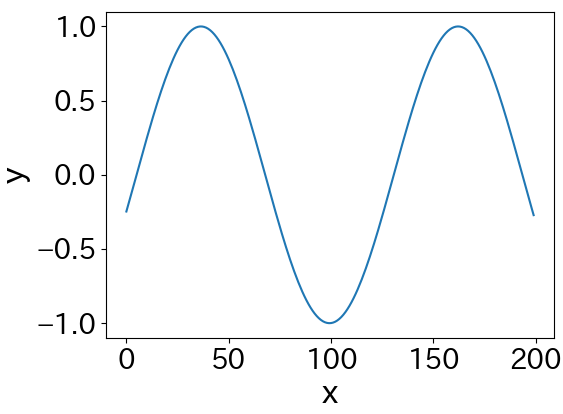
\includegraphics[width=13cm]{./fig/sin}
    \caption{実験に用いた$sin$波}
    \label{fig:sin}
  \end{center}
\end{figure}

\subsection{学習方法}
学習は以下のフローチャートのように行った。
\begin{figure}[ht]
  \begin{center}
    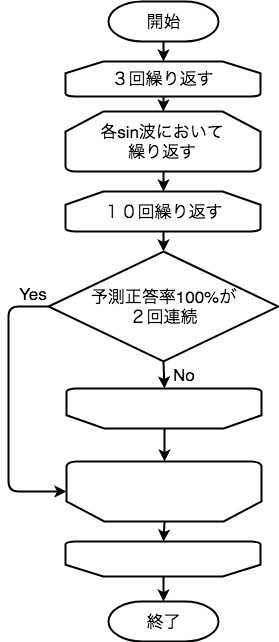
\includegraphics[width=6cm]{./fig/drawing_flow}
    \caption{学習のフローチャート}
    \label{fig:flow_chart}
  \end{center}
\end{figure}

学習方法はHTMに複数のデータを学習をさせる際に1つのデータにおけるセル間の接続を確立するために考案した。
まず1つの$sin$波を10回繰り返して入力することでその$sin$波に対してのHTMの学習を安定させる。
また予測正答率が100\%に2回連続で到達した時点で学習が完了したとみなし、途中で繰り返しを抜ける。
この学習をすべてのデータに対して順に行う。
そしてすべてのデータに対して学習を行った後、また始めのデータに戻り学習を行う。
これを3回繰り返す。
途中で繰り返しを抜けなかった場合の学習全体でのエポック数は150回となる。

この学習方法は人間における暗記学習を模している。
複数の物事を覚えるときに1つの物事を複数回反芻することで定着させようとする。また全体を一度暗記したら復習を繰り返すことで忘却しにくくする。

\subsection{評価指標}
本実験の評価指標はサンプルデータ数200の$sin$波において、最初の1個のデータを入力したあとに、残りの199個のデータを予測した際の正答率である。

\subsection{実験結果}
本実験における各エポックでのそれぞれの条件での予測正答率を以下の図4.2,4.3に示す。

\begin{figure}[ht]
  \begin{center}
    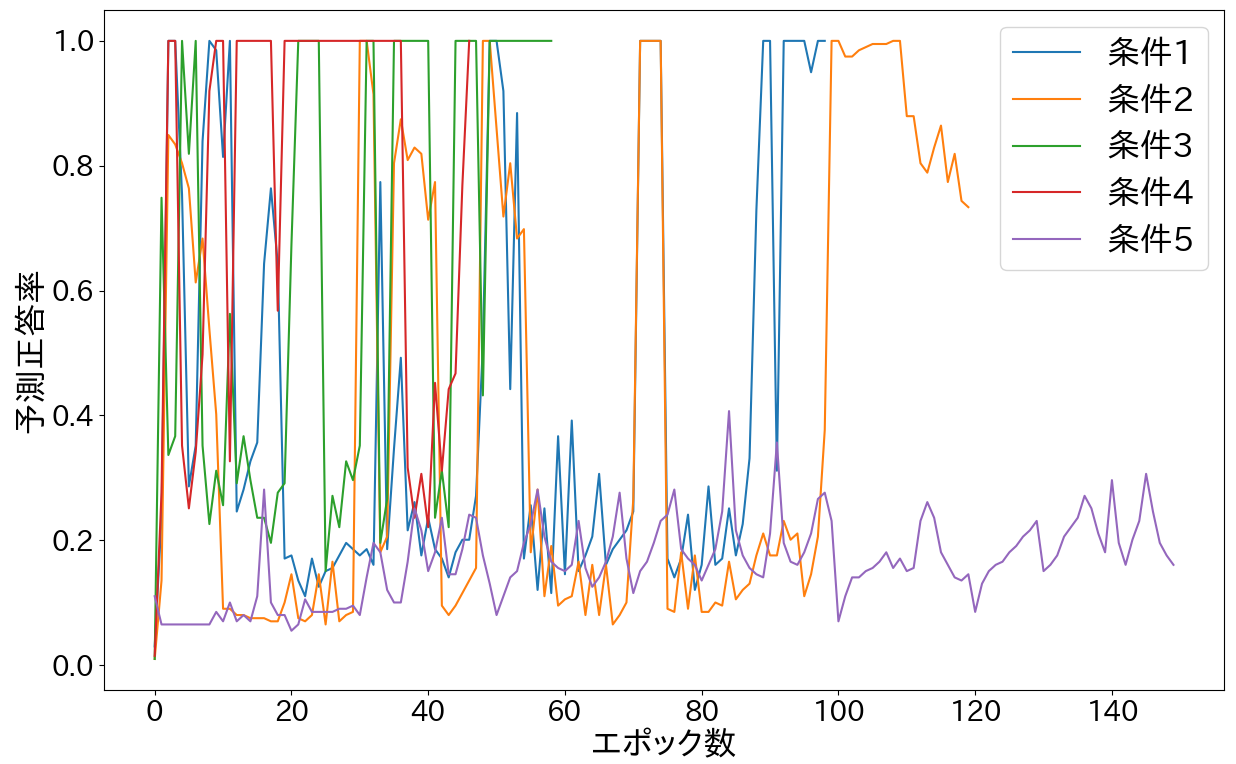
\includegraphics[width=12cm]{./fig/experiment1}
    \caption{実験1の結果1}
    \label{fig:experiment1-1}
  \end{center}
\end{figure}

\begin{figure}[ht]
  \begin{center}
    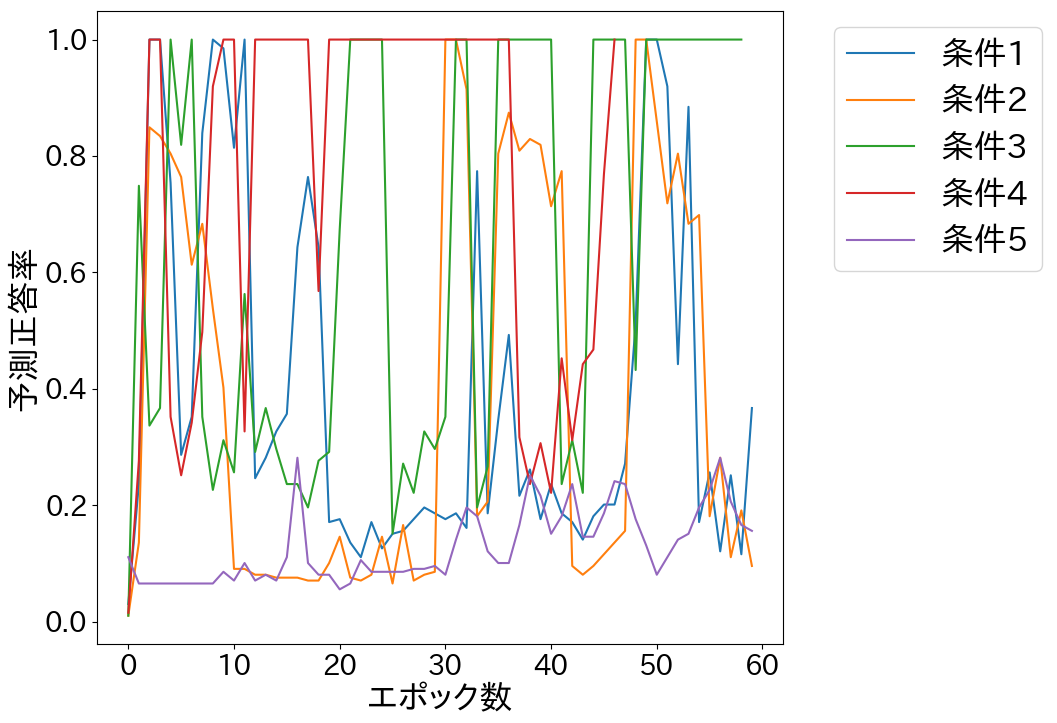
\includegraphics[width=14cm]{./fig/experiment2}
    \caption{実験1の結果2}
    \label{fig:experiment1-2}
  \end{center}
\end{figure}

図4.3は全エポック数における予測正答率を示していて、図4.4は60エポックまでの予測正答率を示している。
HTMの学習における予測正答率は学習の途中においては大きく変化し、最終的には学習によってセル間の接続が確立され、予測正答率が100\%に近づいていく。
条件3と条件4は60エポックまでで学習が完了しており、条件1と条件2は150エポック周辺で学習が完了している。また条件5は最後まで学習が完了しなかった。

次に学習完了後に学習に用いた5つの$sin$波の予測正答率をしたの表4.3に示す。

\begin{table}[hbtp]
  \caption{各通りにおける最終予測正答率}
  \label{htm_predict}
  \centering
  \begin{tabular}{c|l|rrrrr}
    \hline
    \multicolumn{2}{c|}{} & \multicolumn{5}{c}{各条件における予測正答率(\%)} \\
    \hline
    \multicolumn{2}{c|}{} & 1 & 2 & 3 & 4 & 5 \\
    \hline \hline
    \multirow{5}{*}{\rotatebox[origin=c]{90}{各$sin$波}}
    & 1 & 9.0 & 5.5 & 100 & 38.7 & 0.0 \\
    & 2 & 100 & 74.9 & 100 & 16.1 & 13.6 \\
    & 3 & 100 & 13.6 & 100 & 21.6 & 7.5 \\
    & 4 & 100 & 31.2 & 100 & 15.6 & 8.0 \\
    & 5 & 100 & 73.4 & 100 & 100 & 16.1 \\ \hline
    & 平均 & 81.8 & 39.7 & 100 & 38.4 & 9.0 \\
    \hline
  \end{tabular}
\end{table}

表4.3より条件3において最も高い予測精度が記録された。
また条件5で最も低い予測精度となった。

\newpage
\subsection{実験考察}
本実験には以下の3つの傾向が現れた。

\begin{enumerate}
  \item カラム数の減少は性能の低下に大きく影響する。
  \item セル数やセグメント数の減少は性能の低下に影響する。
  \item 時間軸長の増加は性能の向上に影響する。
\end{enumerate}

1つ目に関しては、カラム数がパターンの表現に直接影響することによるものだと考えられる。
2.2.2で述べたようにHTMにおけるパターンの表現はカラムの組み合わせによるものである。
カラム数が少なくなると各パターンを表現するカラムに重複するものが多くなる。
それによってパターンの誤予測が多くなり、HTMの性能が低下する。

2つ目に関しては、セル数やセグメント数は学習の柔軟性に関わる部分であるため、少しの減少では学習の精度に影響することはないのだと考えられる。
しかし条件4のようにセル数とセグメント数の両方を大きく減少させた際に複数のデータを学習すると、セル間の接続の繋がりに偏りが生まれるため、最終的な予測精度が減少すると考えられる。

3つ目に関しては本研究で導入したものであるが、性能の向上に貢献することがわかった。
時間軸長が長いほど性能が高いため、セル数とセグメント数の減少による性能低下が現れない程度にセル数とセグメント数の分の要素数を時間軸長に割り当てたモデルが最も良いと考えられる。

これらの3つの傾向から以降の実験では条件3のモデルを用いる。

\section{実験2}
\subsection{実験目的}
改良型HTMにおける長期依存考慮の性能検証を行った。

\subsection{実験概要}
合成関数を学習させた提案モデルを従来型のHTMや機械学習による手法と比較し、長期依存考慮における性能を検証した。

\subsection{実験条件}

\begin{itemize}
  \item 提案モデル
  \item 従来型HTM
  \item RNN
  \item LSTM
  \item GRU \cite{GRU}
\end{itemize}

\subsection{実験データ}
本実験における学習データとして以下のような合成関数を用いた。

\begin{equation}
    \sin(x) + \frac{1}{2}\cos(2x) + \frac{1}{3}\sin(4x) + \frac{1}{4}\sin(\frac{x}{4})
\end{equation}

\begin{figure}[ht]
  \begin{center}
    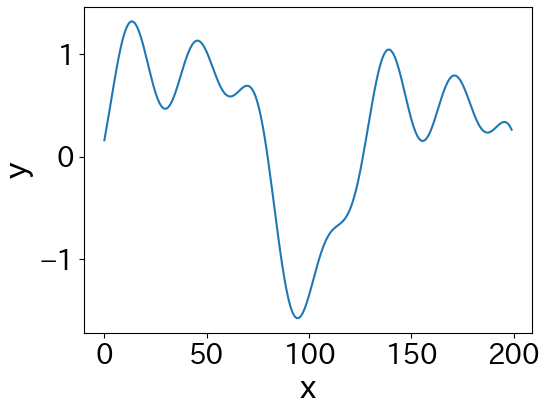
\includegraphics[width=14cm]{./fig/cfunc}
    \caption{実験に用いた合成関数}
    \label{fig:cfunc}
  \end{center}
\end{figure}

\subsection{学習方法}
学習方法は実験1と同様に図4.2のように行った。

\subsection{評価指標}
本実験の評価は、学習に用いたものとは位相をずらした異なったものを用いた。
評価指標はサンプルデータ数200の合成関数において、最初の1個のデータを入力したあとに、残りの199個のデータを予測した際の予測値と正解データとの誤差である。
誤差は各時刻あたりの誤差の絶対値をとり、サンプルデータ数で割り、1時刻あたりの予測誤差を計算したものを用いた。

\newpage
\subsection{実験結果}

\begin{figure}[ht]
  \begin{center}
    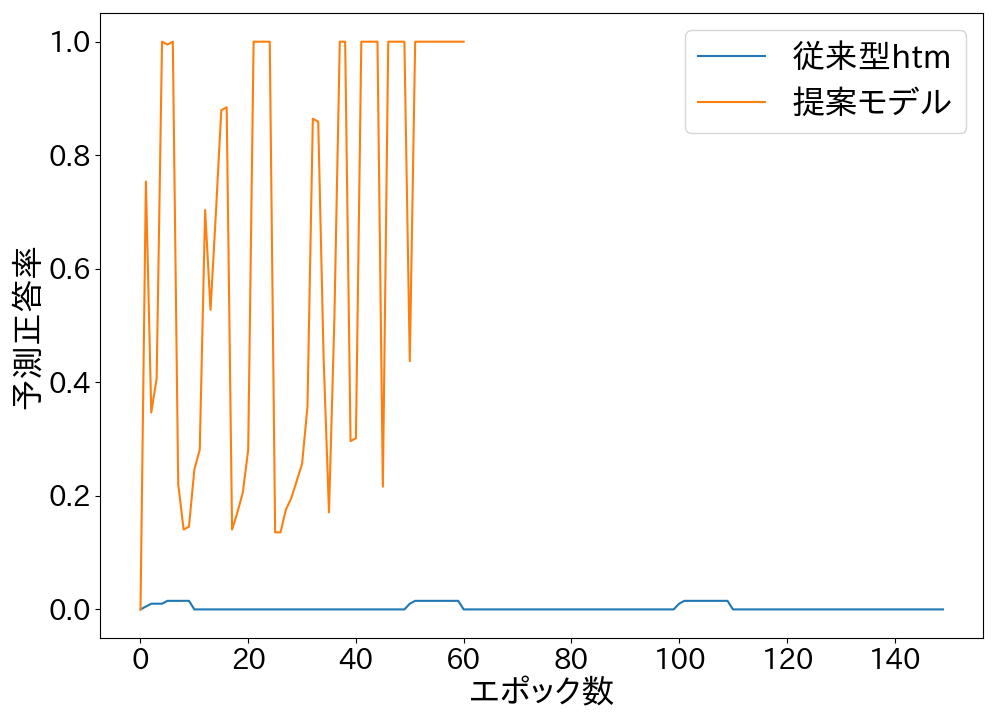
\includegraphics[width=14cm]{./fig/experiment3}
    \caption{実験2の結果}
    \label{fig:experiment2}
  \end{center}
\end{figure}

\begin{table}[hbtp]
  \caption{各モデルにおける結果}
  \label{experiment2}
  \centering
  \begin{tabular}{c|ccccc}
    \hline
    & 提案モデル & 従来型HTM & RNN & LSTM & GRU \\
    \hline \hline
    予測可能時間 & 200 & 28 & 200 & 200 & 200 \\\hline
    \shortstack{\\1時刻あたりの\\予測誤差(絶対値)} & 0.0 & 0.0 & 0.835 & 0.560 & 0.720 \\
    \hline
  \end{tabular}
\end{table}

提案モデルは従来型HTMよりも予測正答率が高くなっていることからもわかるように予測可能時刻が大幅に改善している。
RNNやLSTM、GRUといった機械学習による手法では各時刻において誤差が生じているが、HTMでは誤差が生じていない。

以下の図4.7\~4.10は各モデルにおいて合成関数を再現したものである。

\begin{figure}[htp]
  \begin{center}
    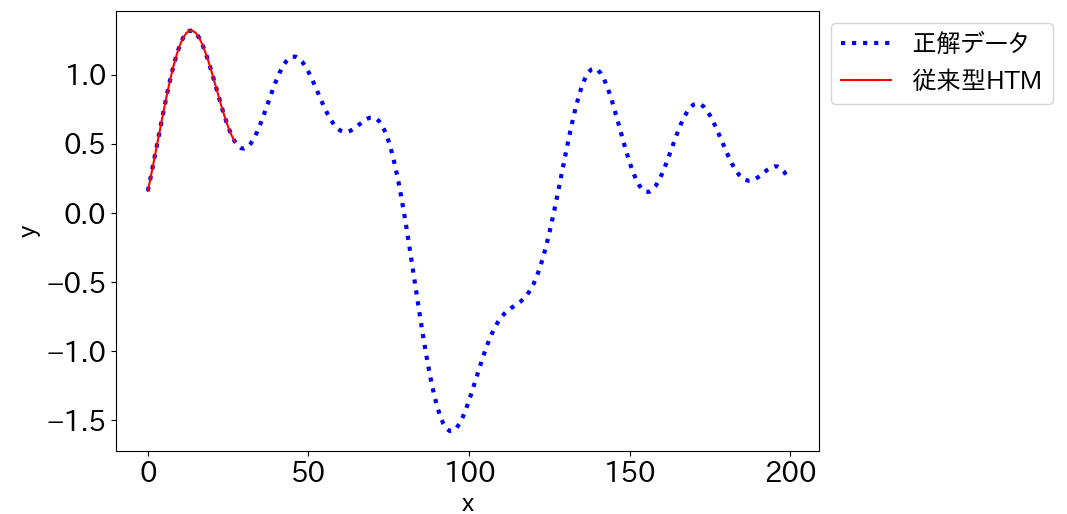
\includegraphics[width=14cm]{./fig/htm}
    \caption{従来型HTMを用いた合成関数の再現}
    \label{fig:htm_experiment2}
  \end{center}
\end{figure}

\begin{figure}[hp]
  \begin{center}
    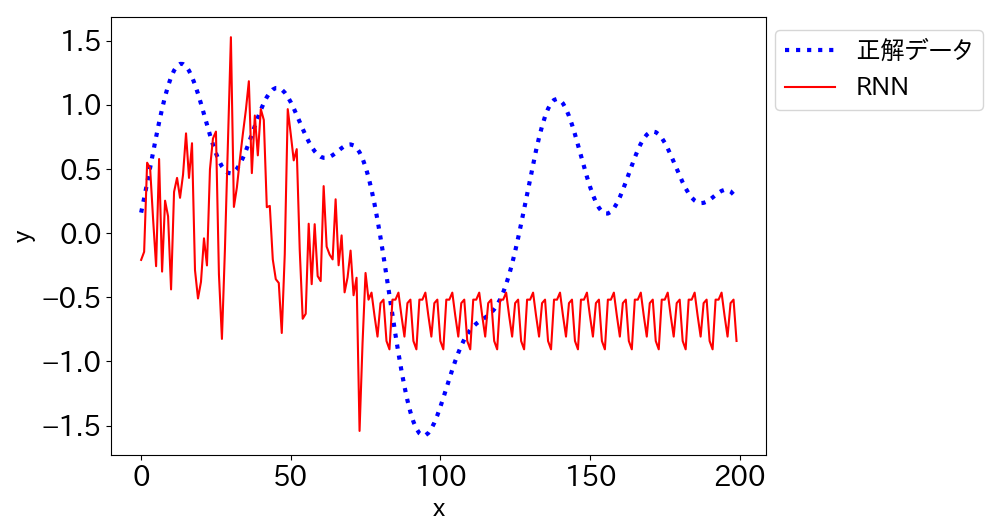
\includegraphics[width=14cm]{./fig/rnn}
    \caption{RNNを用いた合成関数の再現}
    \label{fig:rnn_experiment2}
  \end{center}
\end{figure}

\begin{figure}[htp]
  \begin{center}
    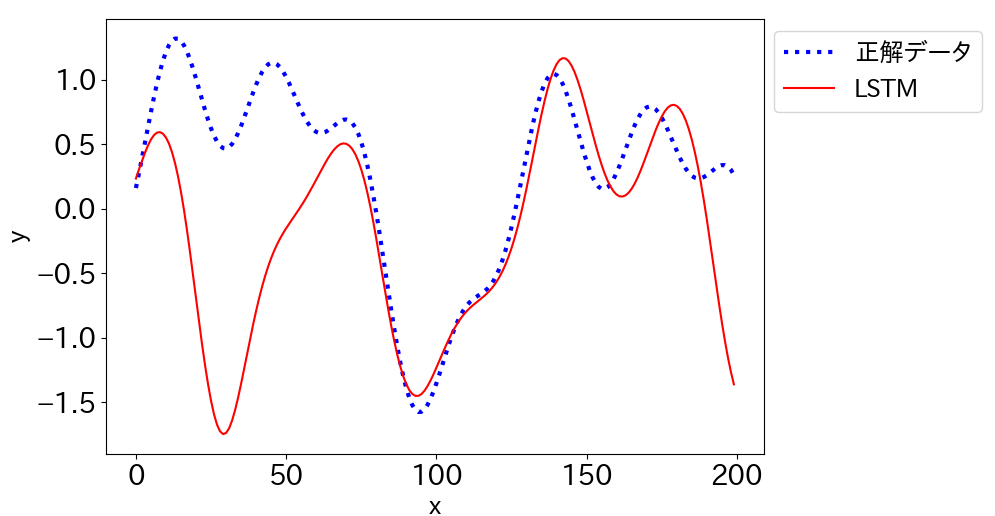
\includegraphics[width=14cm]{./fig/lstm}
    \caption{LSTMを用いた合成関数の再現}
    \label{fig:lstm_experiment2}
  \end{center}
\end{figure}

\begin{figure}[hp]
  \begin{center}
    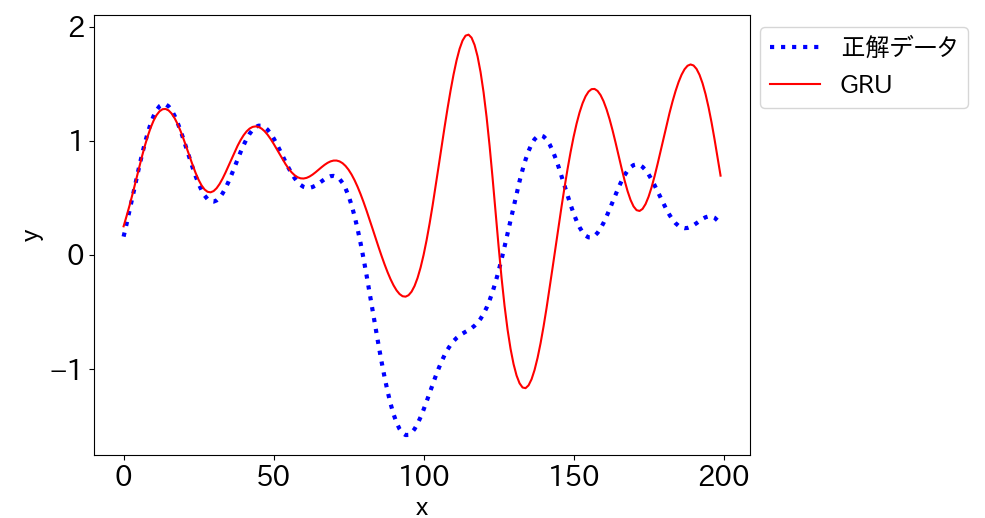
\includegraphics[width=14cm]{./fig/gru}
    \caption{GRUを用いた合成関数の再現}
    \label{fig:gru_experiment2}
  \end{center}
\end{figure}

\begin{figure}[ht]
  \begin{center}
    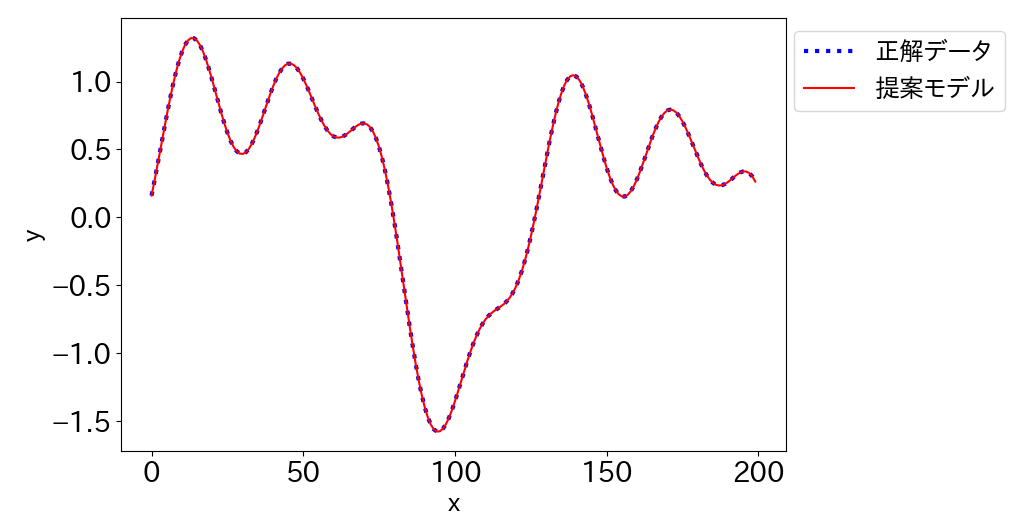
\includegraphics[width=14cm]{./fig/ihtm}
    \caption{提案モデルを用いた合成関数の再現}
    \label{fig:ihtm_experiment2}
  \end{center}
\end{figure}

\newpage
\vspace{3cm}
\subsection{実験考察}
本実験によって以下の2つの考察が考えられる。
\begin{enumerate}
  \item 提案モデルは長期依存関係の考慮において従来型HTMの性能を向上させていると言える。
  \item 提案モデルは機械学習による手法と比較して高い時系列予測精度をもっているため予測誤差がほとんどなくなるような予測ができると言える。
\end{enumerate}
1つ目に関しては、2章で述べた以下の2つの問題を改善したためだと考えられる。
\begin{itemize}
  \item[a.] 疎な分散表現を用いたために発火するセルが徐々に少なくなり消失する。
  \item[b.] 学習が大きく進んだパターンにおいて表現が疎になった時に次のパターンに繋がっていたセルが消失するために学習状態が損失する。
\end{itemize}
特にaの問題において大きい改善があったと考えられる。
これは複数の時刻前のデータとの接続を学習し、予測の際にすべての時刻における予測状態のセルを等価に扱ったことによる。
これにより予測状態のセルの数が従来型HTMよりも多くなり、かつ予測状態のセルの計算が各時刻に分散することで過学習も防ぐことができた。
bの問題は予測精度が最も低かった実験1の条件5の場合においてのみ発生しており、モデルの精度がある程度高い場合においてはbの問題よりもaの問題の方が予測精度に大きく寄与しているものと考えられる。

2つ目に関しては、提案モデルと従来型の両方HTMの予測精度が高いために誤差が0になっていると考えられる。
実験1の条件3以外のモデルでは誤予測があったためHTMにおいてもモデルの精度が低いときに大きく予測が異なる場合があると考えられる。
また今回は各データをランダムなカラムの組み合わせに変換しているため、連続した値でもHTMも表現上では大きく異なったものとなる。
これによって誤予測が起きた場合にその誤差が大きくなるという問題がある。
この問題はHTMのカラムの出力と入力値が近い表現になるように学習する機構を導入することで改善できると思われるため今後の課題としたい。

% \chapter{結論}
本論文では、HTMを複数前の時刻におけるパターンを表現するセルとの接続も持つように改良することを提案した。
HTMの構造の面では接続セグメントに時間軸を導入した。
またHTMの学習アルゴリズムの面では、シナプス接続において複数時刻に渡るセルの発火との関係を持つことと予測状態のセルの計算において複数時刻からの繋がりの重ね合わせを行うことで、長期依存関係を保持することに成功した。
これによって並列予測を要する時系列データに対しての予測タスクにおいて、従来のHTMよりも高い精度を記録することが確認された。

今後の展望として、分散表現をHTMのカラム表現に変換する方法を確立することと、単語分散表現を用いることで自然言語処理における様々な言語モデルに適応することを考えている。
これによって脳の言語処理における語彙を司る分野と文脈を司る分野に分けた学習を模した言語学習が可能になると考えられる。

% \addcontentsline{toc}{chapter}{謝辞}
\chapter*{謝辞}
本研究を行うにあたり、指導教官の萩原将文教授から終始熱心なご指導を承りました。ここに感謝の意を表します。また研究室の方々には様々な相談をさせて頂き、特に武内先輩、米倉先輩、和田先輩には研究を通じて活発な議論にお付き合い頂きましたことを感謝致します。


% \bibliographystyle{jplain}
% \bibliographystyle{jecon.bst}
% \bibliography{./reference/reference}

% \appendix

% \chapter*{付録 A \\ \vspace{7mm} HTMのパラメータ}

% \chapter{HTMの実装}
実装時に用いたHTMのパラメータは以下の表の通りである。

\begin{table}[hbtp]
  \caption{HTMのパラメータ}
  \label{impl_htm_parameter}
  \centering
  \begin{tabular}{c|r}
    パラメータ名 & 値 \\
    \hline \hline
    カラム数 & 512 \\
    1カラム内のセル数 & 16 \\
    1セル内の接続セグメント数 & 32 \\
    予測状態に遷移するのに必要な接続セグメント & 4 \\
    セルの接続値の初期値 & 0.21 \\
    セルにおける接続のしきい値 & 0.5 \\
    接続値を増やす場合の更新式 & 0.1 \\
    接続値を減らす場合の更新式 & 0.1 \\
    予測状態にあったが活性化しなかったセルにおける更新式 & 0.01 \\
    1ステップ内で新たに持てる接続値の最大数 & 32 \\
    \hline
  \end{tabular}
\end{table}


提案モデルと従来型HTMの両方においてpythonによるスクラッチ実装を行った。
ライブラリはnumpyとpytorchのみでpytorchはSparseTensorのみを用いた。
HTMの活性化状態のセルと予測状態のセルはともに疎な分散表現となるためSparseTensorを用いて実装した。
また活性化状態のセルと予測状態のセルからカラム単位での活性化状態の遷移を記録し、それを用いて学習の分岐を行った。
セグメント集合は従来型は5次元、提案モデルは6次元のテンソルを正規分布によってランダムに初期化して用いた。

% \chapter{追加実験}

\end{document}
